\section{Einleitung}
\subsection{Erstes Unterkapitel}
Dies ist ein Zitat:
\lipsum[1-2]
Zwar nicht aus diesem Buch, aber hier eine Zitierung. \citep[vgl. ][S. 5-6]{bernstein97}
\subsection{Zweites Unterkapitel}
Unter Bild \ref{pic:bildname} sieht man eine volle Schönheit.
\begin{figure}[ht]
	\centering
	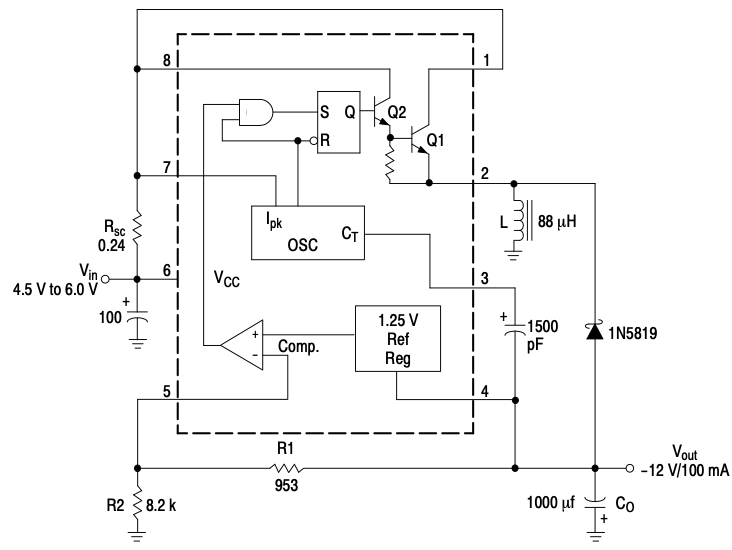
\includegraphics[scale=0.5]{pic/bildname}
	\caption{Beispielbild}
	\label{pic:bildname}
	\quelle \citep[S. 8]{onsemi:MC34063A}
\end{figure}

Eine mögliche Abkürzung ist \ac{cad}. Wenn man dies aber ein zweites Mal schreibt, steht nur noch kurz \ac{cad} da.
\subsection{Drittes Unterkapitel}
\section{Neuer Abschnitt}
\lipsum[1-3]\\

Zum Abschluss soll noch eine Tabelle dargestellt werden:
\begin{table}[H]
\centering
\begin{tabular}{c c}
Zelle 11 & Zelle 12\\
Zelle 21 & Zelle 22\\
\end{tabular}
\caption{Eine Tabelle}
\label{tab:einetabelle}
\quelle Unbekannt
\end{table}